\documentclass[11pt,]{article}
\usepackage{lmodern}
\usepackage{amssymb,amsmath}
\usepackage{ifxetex,ifluatex}
\usepackage{fixltx2e} % provides \textsubscript
\ifnum 0\ifxetex 1\fi\ifluatex 1\fi=0 % if pdftex
  \usepackage[T1]{fontenc}
  \usepackage[utf8]{inputenc}
\else % if luatex or xelatex
  \ifxetex
    \usepackage{mathspec}
  \else
    \usepackage{fontspec}
  \fi
  \defaultfontfeatures{Ligatures=TeX,Scale=MatchLowercase}
\fi
% use upquote if available, for straight quotes in verbatim environments
\IfFileExists{upquote.sty}{\usepackage{upquote}}{}
% use microtype if available
\IfFileExists{microtype.sty}{%
\usepackage{microtype}
\UseMicrotypeSet[protrusion]{basicmath} % disable protrusion for tt fonts
}{}
\usepackage[margin = 1.5in]{geometry}
\usepackage{hyperref}
\PassOptionsToPackage{usenames,dvipsnames}{color} % color is loaded by hyperref
\hypersetup{unicode=true,
            pdftitle={Data Wrangling with dplyr},
            pdfauthor={Abhinav Anand, IIMB},
            colorlinks=true,
            linkcolor=blue,
            citecolor=magenta,
            urlcolor=red,
            breaklinks=true}
\urlstyle{same}  % don't use monospace font for urls
\usepackage{color}
\usepackage{fancyvrb}
\newcommand{\VerbBar}{|}
\newcommand{\VERB}{\Verb[commandchars=\\\{\}]}
\DefineVerbatimEnvironment{Highlighting}{Verbatim}{commandchars=\\\{\}}
% Add ',fontsize=\small' for more characters per line
\usepackage{framed}
\definecolor{shadecolor}{RGB}{248,248,248}
\newenvironment{Shaded}{\begin{snugshade}}{\end{snugshade}}
\newcommand{\KeywordTok}[1]{\textcolor[rgb]{0.13,0.29,0.53}{\textbf{#1}}}
\newcommand{\DataTypeTok}[1]{\textcolor[rgb]{0.13,0.29,0.53}{#1}}
\newcommand{\DecValTok}[1]{\textcolor[rgb]{0.00,0.00,0.81}{#1}}
\newcommand{\BaseNTok}[1]{\textcolor[rgb]{0.00,0.00,0.81}{#1}}
\newcommand{\FloatTok}[1]{\textcolor[rgb]{0.00,0.00,0.81}{#1}}
\newcommand{\ConstantTok}[1]{\textcolor[rgb]{0.00,0.00,0.00}{#1}}
\newcommand{\CharTok}[1]{\textcolor[rgb]{0.31,0.60,0.02}{#1}}
\newcommand{\SpecialCharTok}[1]{\textcolor[rgb]{0.00,0.00,0.00}{#1}}
\newcommand{\StringTok}[1]{\textcolor[rgb]{0.31,0.60,0.02}{#1}}
\newcommand{\VerbatimStringTok}[1]{\textcolor[rgb]{0.31,0.60,0.02}{#1}}
\newcommand{\SpecialStringTok}[1]{\textcolor[rgb]{0.31,0.60,0.02}{#1}}
\newcommand{\ImportTok}[1]{#1}
\newcommand{\CommentTok}[1]{\textcolor[rgb]{0.56,0.35,0.01}{\textit{#1}}}
\newcommand{\DocumentationTok}[1]{\textcolor[rgb]{0.56,0.35,0.01}{\textbf{\textit{#1}}}}
\newcommand{\AnnotationTok}[1]{\textcolor[rgb]{0.56,0.35,0.01}{\textbf{\textit{#1}}}}
\newcommand{\CommentVarTok}[1]{\textcolor[rgb]{0.56,0.35,0.01}{\textbf{\textit{#1}}}}
\newcommand{\OtherTok}[1]{\textcolor[rgb]{0.56,0.35,0.01}{#1}}
\newcommand{\FunctionTok}[1]{\textcolor[rgb]{0.00,0.00,0.00}{#1}}
\newcommand{\VariableTok}[1]{\textcolor[rgb]{0.00,0.00,0.00}{#1}}
\newcommand{\ControlFlowTok}[1]{\textcolor[rgb]{0.13,0.29,0.53}{\textbf{#1}}}
\newcommand{\OperatorTok}[1]{\textcolor[rgb]{0.81,0.36,0.00}{\textbf{#1}}}
\newcommand{\BuiltInTok}[1]{#1}
\newcommand{\ExtensionTok}[1]{#1}
\newcommand{\PreprocessorTok}[1]{\textcolor[rgb]{0.56,0.35,0.01}{\textit{#1}}}
\newcommand{\AttributeTok}[1]{\textcolor[rgb]{0.77,0.63,0.00}{#1}}
\newcommand{\RegionMarkerTok}[1]{#1}
\newcommand{\InformationTok}[1]{\textcolor[rgb]{0.56,0.35,0.01}{\textbf{\textit{#1}}}}
\newcommand{\WarningTok}[1]{\textcolor[rgb]{0.56,0.35,0.01}{\textbf{\textit{#1}}}}
\newcommand{\AlertTok}[1]{\textcolor[rgb]{0.94,0.16,0.16}{#1}}
\newcommand{\ErrorTok}[1]{\textcolor[rgb]{0.64,0.00,0.00}{\textbf{#1}}}
\newcommand{\NormalTok}[1]{#1}
\usepackage{graphicx,grffile}
\makeatletter
\def\maxwidth{\ifdim\Gin@nat@width>\linewidth\linewidth\else\Gin@nat@width\fi}
\def\maxheight{\ifdim\Gin@nat@height>\textheight\textheight\else\Gin@nat@height\fi}
\makeatother
% Scale images if necessary, so that they will not overflow the page
% margins by default, and it is still possible to overwrite the defaults
% using explicit options in \includegraphics[width, height, ...]{}
\setkeys{Gin}{width=\maxwidth,height=\maxheight,keepaspectratio}
\IfFileExists{parskip.sty}{%
\usepackage{parskip}
}{% else
\setlength{\parindent}{0pt}
\setlength{\parskip}{6pt plus 2pt minus 1pt}
}
\setlength{\emergencystretch}{3em}  % prevent overfull lines
\providecommand{\tightlist}{%
  \setlength{\itemsep}{0pt}\setlength{\parskip}{0pt}}
\setcounter{secnumdepth}{0}
% Redefines (sub)paragraphs to behave more like sections
\ifx\paragraph\undefined\else
\let\oldparagraph\paragraph
\renewcommand{\paragraph}[1]{\oldparagraph{#1}\mbox{}}
\fi
\ifx\subparagraph\undefined\else
\let\oldsubparagraph\subparagraph
\renewcommand{\subparagraph}[1]{\oldsubparagraph{#1}\mbox{}}
\fi

%%% Use protect on footnotes to avoid problems with footnotes in titles
\let\rmarkdownfootnote\footnote%
\def\footnote{\protect\rmarkdownfootnote}

%%% Change title format to be more compact
\usepackage{titling}

% Create subtitle command for use in maketitle
\newcommand{\subtitle}[1]{
  \posttitle{
    \begin{center}\large#1\end{center}
    }
}

\setlength{\droptitle}{-2em}
  \title{Data Wrangling with \texttt{dplyr}}
  \pretitle{\vspace{\droptitle}\centering\huge}
  \posttitle{\par}
  \author{Abhinav Anand, IIMB}
  \preauthor{\centering\large\emph}
  \postauthor{\par}
  \predate{\centering\large\emph}
  \postdate{\par}
  \date{2018/06/08}

\linespread{1.25}

\begin{document}
\maketitle

\section{Setup}\label{setup}

The package suite \texttt{tidyverse()} which includes the package
\texttt{dplyr} needs to be included. Also, the package
\texttt{gapminder} needs to be installed prior to running the commands
below. For installing \texttt{dplyr}, type
\texttt{install.packages("dplyr")} or equivalently for
\texttt{tidyverse}, type \texttt{install.packages("tidyverse")}. To
install \texttt{gapminder}, type \texttt{install.packages("gapminder")}
in the RStudio console.

\begin{Shaded}
\begin{Highlighting}[]
\NormalTok{(data_gapminder <-}\StringTok{ }\NormalTok{gapminder}\OperatorTok{::}\NormalTok{gapminder)}
\end{Highlighting}
\end{Shaded}

\begin{verbatim}
## # A tibble: 1,704 x 6
##    country     continent  year lifeExp      pop gdpPercap
##    <fct>       <fct>     <int>   <dbl>    <int>     <dbl>
##  1 Afghanistan Asia       1952    28.8  8425333      779.
##  2 Afghanistan Asia       1957    30.3  9240934      821.
##  3 Afghanistan Asia       1962    32.0 10267083      853.
##  4 Afghanistan Asia       1967    34.0 11537966      836.
##  5 Afghanistan Asia       1972    36.1 13079460      740.
##  6 Afghanistan Asia       1977    38.4 14880372      786.
##  7 Afghanistan Asia       1982    39.9 12881816      978.
##  8 Afghanistan Asia       1987    40.8 13867957      852.
##  9 Afghanistan Asia       1992    41.7 16317921      649.
## 10 Afghanistan Asia       1997    41.8 22227415      635.
## # ... with 1,694 more rows
\end{verbatim}

\begin{Shaded}
\begin{Highlighting}[]
\CommentTok{#what is the format: wide or long?}
\CommentTok{#what is a tibble?}
\end{Highlighting}
\end{Shaded}

\subsubsection{Notes}\label{notes}

\begin{enumerate}
\def\labelenumi{\arabic{enumi}.}
\tightlist
\item
  \textbf{Data Types}: R has many in-built data types. Examples:

  \begin{enumerate}
  \def\labelenumii{\roman{enumii}.}
  \tightlist
  \item
    \texttt{fct}: ``factor'': categorical data which can assume finite
    levels, say A, B, C etc.
  \item
    \texttt{dbl}: ``double'': real numbers, say 3.671, 4.00,
    10.122482929 etc.
  \item
    \texttt{int}: ``integer'': integers, say 3, 10, -9, 0 etc.
  \item
    \texttt{chr}: ``character'': say, ``FMC'', ``Term 4'' etc.
  \item
    \texttt{lgl}: ``logical'': \(\{0, 1\}\equiv \{\text{T, F}\}\)
  \item
    \texttt{date}, and many more
  \end{enumerate}
\item
  \textbf{Tibbles}: Tibbles are essentially data frames, but slightly
  altered to work better in tidyverse. (Compare
  \texttt{head(data\_frame\_name)} versus \texttt{tibble\_name}.)
\end{enumerate}

\section{\texorpdfstring{\texttt{dplyr()}: The Main
Verbs}{dplyr(): The Main Verbs}}\label{dplyr-the-main-verbs}

\begin{enumerate}
\def\labelenumi{\arabic{enumi}.}
\tightlist
\item
  \texttt{filter()}: Extract rows
\item
  \texttt{select()}: Extract columns
\item
  \texttt{arrange()}: Order rows
\item
  \texttt{mutate()}: Create new columns (= variables)
\item
  \texttt{summarise()}: Compute summary statistics
\end{enumerate}

The syntax for all five verbs is similar. The first argument is the data
frame, followed by the action to be performed using the variable name.

\subsection{Filter}\label{filter}

Let us observe the state of the world in 1952 and the contrast and
compare with that in 2007.

\begin{Shaded}
\begin{Highlighting}[]
\NormalTok{(data_}\DecValTok{1952}\NormalTok{ <-}\StringTok{ }\NormalTok{data_gapminder }\OperatorTok
\StringTok{  }\NormalTok{dplyr}\OperatorTok{::}\KeywordTok{filter}\NormalTok{(year }\OperatorTok{==}\StringTok{ }\DecValTok{1952}\NormalTok{) }\CommentTok{#extract the rows for year 1952}
\NormalTok{ ) }\CommentTok{#note == as opposed to =}
\end{Highlighting}
\end{Shaded}

\begin{verbatim}
## # A tibble: 142 x 6
##    country     continent  year lifeExp      pop gdpPercap
##    <fct>       <fct>     <int>   <dbl>    <int>     <dbl>
##  1 Afghanistan Asia       1952    28.8  8425333      779.
##  2 Albania     Europe     1952    55.2  1282697     1601.
##  3 Algeria     Africa     1952    43.1  9279525     2449.
##  4 Angola      Africa     1952    30.0  4232095     3521.
##  5 Argentina   Americas   1952    62.5 17876956     5911.
##  6 Australia   Oceania    1952    69.1  8691212    10040.
##  7 Austria     Europe     1952    66.8  6927772     6137.
##  8 Bahrain     Asia       1952    50.9   120447     9867.
##  9 Bangladesh  Asia       1952    37.5 46886859      684.
## 10 Belgium     Europe     1952    68    8730405     8343.
## # ... with 132 more rows
\end{verbatim}

\begin{Shaded}
\begin{Highlighting}[]
\NormalTok{(data_}\DecValTok{2007}\NormalTok{ <-}\StringTok{ }\NormalTok{data_gapminder }\OperatorTok
\StringTok{  }\NormalTok{dplyr}\OperatorTok{::}\KeywordTok{filter}\NormalTok{(year }\OperatorTok{==}\StringTok{ }\DecValTok{2007}\NormalTok{) }\CommentTok{#extract the rows for year 2007}
\NormalTok{ )}
\end{Highlighting}
\end{Shaded}

\begin{verbatim}
## # A tibble: 142 x 6
##    country     continent  year lifeExp       pop gdpPercap
##    <fct>       <fct>     <int>   <dbl>     <int>     <dbl>
##  1 Afghanistan Asia       2007    43.8  31889923      975.
##  2 Albania     Europe     2007    76.4   3600523     5937.
##  3 Algeria     Africa     2007    72.3  33333216     6223.
##  4 Angola      Africa     2007    42.7  12420476     4797.
##  5 Argentina   Americas   2007    75.3  40301927    12779.
##  6 Australia   Oceania    2007    81.2  20434176    34435.
##  7 Austria     Europe     2007    79.8   8199783    36126.
##  8 Bahrain     Asia       2007    75.6    708573    29796.
##  9 Bangladesh  Asia       2007    64.1 150448339     1391.
## 10 Belgium     Europe     2007    79.4  10392226    33693.
## # ... with 132 more rows
\end{verbatim}

\subsection{Select}\label{select}

Let us also focus on two variables---GDP/capita and life expectancy. We
extract both for years 1952 and 2007.

\begin{Shaded}
\begin{Highlighting}[]
\NormalTok{(data_1952_gdppc <-}\StringTok{ }\NormalTok{data_}\DecValTok{1952} \OperatorTok
\StringTok{  }\NormalTok{dplyr}\OperatorTok{::}\KeywordTok{select}\NormalTok{(country, year, gdpPercap)}
\NormalTok{ )}
\end{Highlighting}
\end{Shaded}

\begin{verbatim}
## # A tibble: 142 x 3
##    country      year gdpPercap
##    <fct>       <int>     <dbl>
##  1 Afghanistan  1952      779.
##  2 Albania      1952     1601.
##  3 Algeria      1952     2449.
##  4 Angola       1952     3521.
##  5 Argentina    1952     5911.
##  6 Australia    1952    10040.
##  7 Austria      1952     6137.
##  8 Bahrain      1952     9867.
##  9 Bangladesh   1952      684.
## 10 Belgium      1952     8343.
## # ... with 132 more rows
\end{verbatim}

\begin{Shaded}
\begin{Highlighting}[]
\NormalTok{(data_2007_gdppc <-}\StringTok{ }\NormalTok{data_}\DecValTok{2007} \OperatorTok
\StringTok{  }\NormalTok{dplyr}\OperatorTok{::}\KeywordTok{select}\NormalTok{(country, year, gdpPercap)}
\NormalTok{ )}
\end{Highlighting}
\end{Shaded}

\begin{verbatim}
## # A tibble: 142 x 3
##    country      year gdpPercap
##    <fct>       <int>     <dbl>
##  1 Afghanistan  2007      975.
##  2 Albania      2007     5937.
##  3 Algeria      2007     6223.
##  4 Angola       2007     4797.
##  5 Argentina    2007    12779.
##  6 Australia    2007    34435.
##  7 Austria      2007    36126.
##  8 Bahrain      2007    29796.
##  9 Bangladesh   2007     1391.
## 10 Belgium      2007    33693.
## # ... with 132 more rows
\end{verbatim}

\begin{Shaded}
\begin{Highlighting}[]
\NormalTok{(data_1952_life_exp <-}\StringTok{ }\NormalTok{data_}\DecValTok{1952} \OperatorTok
\StringTok{  }\NormalTok{dplyr}\OperatorTok{::}\KeywordTok{select}\NormalTok{(country, year, lifeExp)}
\NormalTok{ )}
\end{Highlighting}
\end{Shaded}

\begin{verbatim}
## # A tibble: 142 x 3
##    country      year lifeExp
##    <fct>       <int>   <dbl>
##  1 Afghanistan  1952    28.8
##  2 Albania      1952    55.2
##  3 Algeria      1952    43.1
##  4 Angola       1952    30.0
##  5 Argentina    1952    62.5
##  6 Australia    1952    69.1
##  7 Austria      1952    66.8
##  8 Bahrain      1952    50.9
##  9 Bangladesh   1952    37.5
## 10 Belgium      1952    68  
## # ... with 132 more rows
\end{verbatim}

\begin{Shaded}
\begin{Highlighting}[]
\NormalTok{(data_2007_life_exp <-}\StringTok{ }\NormalTok{data_}\DecValTok{2007} \OperatorTok
\StringTok{  }\NormalTok{dplyr}\OperatorTok{::}\KeywordTok{select}\NormalTok{(country, year, lifeExp)}
\NormalTok{ )}
\end{Highlighting}
\end{Shaded}

\begin{verbatim}
## # A tibble: 142 x 3
##    country      year lifeExp
##    <fct>       <int>   <dbl>
##  1 Afghanistan  2007    43.8
##  2 Albania      2007    76.4
##  3 Algeria      2007    72.3
##  4 Angola       2007    42.7
##  5 Argentina    2007    75.3
##  6 Australia    2007    81.2
##  7 Austria      2007    79.8
##  8 Bahrain      2007    75.6
##  9 Bangladesh   2007    64.1
## 10 Belgium      2007    79.4
## # ... with 132 more rows
\end{verbatim}

\begin{Shaded}
\begin{Highlighting}[]
\CommentTok{# = dplyr::select(-c(continent, pop, gdpPercap))}
\end{Highlighting}
\end{Shaded}

\texttt{dplyr::rename()} is a wrapper function for \texttt{select()}
which renames the variable in consideration and keeps all other
variables intact.

\subsection{Arrange}\label{arrange}

Usage of \texttt{arrange()} orders (from first to last) entries on the
basis of a variable.

\subsubsection{Question: Is the set of richest countries the same in
1952 and
2007?}\label{question-is-the-set-of-richest-countries-the-same-in-1952-and-2007}

\begin{Shaded}
\begin{Highlighting}[]
\NormalTok{(data_1952_rich <-}\StringTok{ }\NormalTok{data_1952_gdppc }\OperatorTok
\StringTok{  }\NormalTok{dplyr}\OperatorTok{::}\KeywordTok{arrange}\NormalTok{(}\KeywordTok{desc}\NormalTok{(gdpPercap)) }\CommentTok{#note the use of desc()}
\NormalTok{ )}
\end{Highlighting}
\end{Shaded}

\begin{verbatim}
## # A tibble: 142 x 3
##    country         year gdpPercap
##    <fct>          <int>     <dbl>
##  1 Kuwait          1952   108382.
##  2 Switzerland     1952    14734.
##  3 United States   1952    13990.
##  4 Canada          1952    11367.
##  5 New Zealand     1952    10557.
##  6 Norway          1952    10095.
##  7 Australia       1952    10040.
##  8 United Kingdom  1952     9980.
##  9 Bahrain         1952     9867.
## 10 Denmark         1952     9692.
## # ... with 132 more rows
\end{verbatim}

\begin{Shaded}
\begin{Highlighting}[]
\NormalTok{(data_2007_rich <-}\StringTok{ }\NormalTok{data_2007_gdppc }\OperatorTok
\StringTok{  }\NormalTok{dplyr}\OperatorTok{::}\KeywordTok{arrange}\NormalTok{(}\KeywordTok{desc}\NormalTok{(gdpPercap)) }\CommentTok{#note the use of desc()}
\NormalTok{ )}
\end{Highlighting}
\end{Shaded}

\begin{verbatim}
## # A tibble: 142 x 3
##    country           year gdpPercap
##    <fct>            <int>     <dbl>
##  1 Norway            2007    49357.
##  2 Kuwait            2007    47307.
##  3 Singapore         2007    47143.
##  4 United States     2007    42952.
##  5 Ireland           2007    40676.
##  6 Hong Kong, China  2007    39725.
##  7 Switzerland       2007    37506.
##  8 Netherlands       2007    36798.
##  9 Canada            2007    36319.
## 10 Iceland           2007    36181.
## # ... with 132 more rows
\end{verbatim}

\subsubsection{Which countries display the highest life expectancy
pre-2000?}\label{which-countries-display-the-highest-life-expectancy-pre-2000}

\begin{Shaded}
\begin{Highlighting}[]
\NormalTok{(data_life_pre00 <-}\StringTok{ }\NormalTok{data_gapminder }\OperatorTok
\StringTok{  }\NormalTok{dplyr}\OperatorTok{::}\KeywordTok{select}\NormalTok{(country, year, lifeExp) }\OperatorTok
\StringTok{  }\NormalTok{dplyr}\OperatorTok{::}\KeywordTok{filter}\NormalTok{(year }\OperatorTok{<=}\StringTok{ }\DecValTok{2000}\NormalTok{) }\OperatorTok
\StringTok{  }\NormalTok{dplyr}\OperatorTok{::}\KeywordTok{arrange}\NormalTok{(}\KeywordTok{desc}\NormalTok{(lifeExp))}
\NormalTok{ )}
\end{Highlighting}
\end{Shaded}

\begin{verbatim}
## # A tibble: 1,420 x 3
##    country           year lifeExp
##    <fct>            <int>   <dbl>
##  1 Japan             1997    80.7
##  2 Hong Kong, China  1997    80  
##  3 Sweden            1997    79.4
##  4 Switzerland       1997    79.4
##  5 Japan             1992    79.4
##  6 Iceland           1997    79.0
##  7 Australia         1997    78.8
##  8 Italy             1997    78.8
##  9 Iceland           1992    78.8
## 10 Spain             1997    78.8
## # ... with 1,410 more rows
\end{verbatim}

\subsubsection{Post-2000?}\label{post-2000}

\begin{Shaded}
\begin{Highlighting}[]
\NormalTok{(data_life_post00 <-}\StringTok{ }\NormalTok{data_gapminder }\OperatorTok
\StringTok{  }\NormalTok{dplyr}\OperatorTok{::}\KeywordTok{select}\NormalTok{(country, year, lifeExp) }\OperatorTok
\StringTok{  }\NormalTok{dplyr}\OperatorTok{::}\KeywordTok{filter}\NormalTok{(year }\OperatorTok{>}\StringTok{ }\DecValTok{2000}\NormalTok{) }\OperatorTok
\StringTok{  }\NormalTok{dplyr}\OperatorTok{::}\KeywordTok{arrange}\NormalTok{(}\KeywordTok{desc}\NormalTok{(lifeExp))}
\NormalTok{ )}
\end{Highlighting}
\end{Shaded}

\begin{verbatim}
## # A tibble: 284 x 3
##    country           year lifeExp
##    <fct>            <int>   <dbl>
##  1 Japan             2007    82.6
##  2 Hong Kong, China  2007    82.2
##  3 Japan             2002    82  
##  4 Iceland           2007    81.8
##  5 Switzerland       2007    81.7
##  6 Hong Kong, China  2002    81.5
##  7 Australia         2007    81.2
##  8 Spain             2007    80.9
##  9 Sweden            2007    80.9
## 10 Israel            2007    80.7
## # ... with 274 more rows
\end{verbatim}

\subsection{Mutate}\label{mutate}

Let's define a new variable called ``total GDP'' which is the product of
the GDP/capita and the total population. To compute it and include it in
the list of variables we can use the verb \texttt{dplyr::mutate()}.

\begin{Shaded}
\begin{Highlighting}[]
\NormalTok{(data_GDP_tot <-}\StringTok{ }\NormalTok{data_gapminder }\OperatorTok
\StringTok{   }\NormalTok{dplyr}\OperatorTok{::}\KeywordTok{mutate}\NormalTok{(}\DataTypeTok{GDP_total =}\NormalTok{ pop}\OperatorTok{*}\NormalTok{gdpPercap}\OperatorTok{/}\DecValTok{10}\OperatorTok{^}\DecValTok{9}\NormalTok{) }\CommentTok{#in USD billions}
\NormalTok{ )}
\end{Highlighting}
\end{Shaded}

\begin{verbatim}
## # A tibble: 1,704 x 7
##    country     continent  year lifeExp      pop gdpPercap GDP_total
##    <fct>       <fct>     <int>   <dbl>    <int>     <dbl>     <dbl>
##  1 Afghanistan Asia       1952    28.8  8425333      779.      6.57
##  2 Afghanistan Asia       1957    30.3  9240934      821.      7.59
##  3 Afghanistan Asia       1962    32.0 10267083      853.      8.76
##  4 Afghanistan Asia       1967    34.0 11537966      836.      9.65
##  5 Afghanistan Asia       1972    36.1 13079460      740.      9.68
##  6 Afghanistan Asia       1977    38.4 14880372      786.     11.7 
##  7 Afghanistan Asia       1982    39.9 12881816      978.     12.6 
##  8 Afghanistan Asia       1987    40.8 13867957      852.     11.8 
##  9 Afghanistan Asia       1992    41.7 16317921      649.     10.6 
## 10 Afghanistan Asia       1997    41.8 22227415      635.     14.1 
## # ... with 1,694 more rows
\end{verbatim}

In general, for \texttt{mutate()} to work well, the function must take a
vector of values as input and return a vector with the same number of
values as output. A short list of functions that can be used with
\texttt{mutate()} are:

\begin{enumerate}
\def\labelenumi{\arabic{enumi}.}
\tightlist
\item
  Arithmetic operators: \texttt{+}, \texttt{-}, \texttt{*}, \texttt{/},
  \texttt{\^{}}
\item
  Logs: \texttt{log()}, \texttt{log2()}, \texttt{log10()}
\item
  Cumulative aggregates: \texttt{cumsum()}, \texttt{cumprod()},
  \texttt{cummin()}, \texttt{cummax()}, \texttt{cummean()} etc.
\end{enumerate}

and many more.

\subsubsection{Question: Which countries have the highest total GDP in
1952 and
2007?}\label{question-which-countries-have-the-highest-total-gdp-in-1952-and-2007}

\begin{Shaded}
\begin{Highlighting}[]
\NormalTok{(data_GDP_tot }\OperatorTok\StringTok{ }
\StringTok{   }\NormalTok{dplyr}\OperatorTok{::}\KeywordTok{filter}\NormalTok{(year }\OperatorTok{==}\StringTok{ }\DecValTok{1952}\NormalTok{) }\OperatorTok
\StringTok{   }\NormalTok{dplyr}\OperatorTok{::}\KeywordTok{arrange}\NormalTok{(}\KeywordTok{desc}\NormalTok{(GDP_total))}
\NormalTok{ )}
\end{Highlighting}
\end{Shaded}

\begin{verbatim}
## # A tibble: 142 x 7
##    country        continent  year lifeExp       pop gdpPercap GDP_total
##    <fct>          <fct>     <int>   <dbl>     <int>     <dbl>     <dbl>
##  1 United States  Americas   1952    68.4 157553000    13990.     2204.
##  2 United Kingdom Europe     1952    69.2  50430000     9980.      503.
##  3 Germany        Europe     1952    67.5  69145952     7144.      494.
##  4 France         Europe     1952    67.4  42459667     7030.      298.
##  5 Japan          Asia       1952    63.0  86459025     3217.      278.
##  6 Italy          Europe     1952    65.9  47666000     4931.      235.
##  7 China          Asia       1952    44   556263527      400.      223.
##  8 India          Asia       1952    37.4 372000000      547.      203.
##  9 Canada         Americas   1952    68.8  14785584    11367.      168.
## 10 Brazil         Americas   1952    50.9  56602560     2109.      119.
## # ... with 132 more rows
\end{verbatim}

\begin{Shaded}
\begin{Highlighting}[]
\NormalTok{(data_GDP_tot }\OperatorTok\StringTok{ }
\StringTok{   }\NormalTok{dplyr}\OperatorTok{::}\KeywordTok{filter}\NormalTok{(year }\OperatorTok{==}\StringTok{ }\DecValTok{2007}\NormalTok{) }\OperatorTok
\StringTok{   }\NormalTok{dplyr}\OperatorTok{::}\KeywordTok{arrange}\NormalTok{(}\KeywordTok{desc}\NormalTok{(GDP_total))}
\NormalTok{ )}
\end{Highlighting}
\end{Shaded}

\begin{verbatim}
## # A tibble: 142 x 7
##    country        continent  year lifeExp        pop gdpPercap GDP_total
##    <fct>          <fct>     <int>   <dbl>      <int>     <dbl>     <dbl>
##  1 United States  Americas   2007    78.2  301139947    42952.    12934.
##  2 China          Asia       2007    73.0 1318683096     4959.     6540.
##  3 Japan          Asia       2007    82.6  127467972    31656.     4035.
##  4 India          Asia       2007    64.7 1110396331     2452.     2723.
##  5 Germany        Europe     2007    79.4   82400996    32170.     2651.
##  6 United Kingdom Europe     2007    79.4   60776238    33203.     2018.
##  7 France         Europe     2007    80.7   61083916    30470.     1861.
##  8 Brazil         Americas   2007    72.4  190010647     9066.     1723.
##  9 Italy          Europe     2007    80.5   58147733    28570.     1661.
## 10 Mexico         Americas   2007    76.2  108700891    11978.     1302.
## # ... with 132 more rows
\end{verbatim}

\subsubsection{Question: Which are the five smallest economies in 2007
(by total
GDP)?}\label{question-which-are-the-five-smallest-economies-in-2007-by-total-gdp}

\begin{Shaded}
\begin{Highlighting}[]
\NormalTok{(data_GDP_tot }\OperatorTok\StringTok{ }
\StringTok{   }\NormalTok{dplyr}\OperatorTok{::}\KeywordTok{filter}\NormalTok{(year }\OperatorTok{==}\StringTok{ }\DecValTok{2007}\NormalTok{) }\OperatorTok
\StringTok{   }\NormalTok{dplyr}\OperatorTok{::}\KeywordTok{arrange}\NormalTok{(GDP_total) }\OperatorTok
\StringTok{   }\NormalTok{dplyr}\OperatorTok{::}\KeywordTok{filter}\NormalTok{(}\KeywordTok{rank}\NormalTok{(GDP_total) }\OperatorTok{<=}\StringTok{ }\DecValTok{5}\NormalTok{)}
\NormalTok{ )}
\end{Highlighting}
\end{Shaded}

\begin{verbatim}
## # A tibble: 5 x 7
##   country               continent  year lifeExp    pop gdpPercap GDP_total
##   <fct>                 <fct>     <int>   <dbl>  <int>     <dbl>     <dbl>
## 1 Sao Tome and Principe Africa     2007    65.5 2.00e5     1598.     0.319
## 2 Comoros               Africa     2007    65.2 7.11e5      986.     0.701
## 3 Guinea-Bissau         Africa     2007    46.4 1.47e6      579.     0.853
## 4 Djibouti              Africa     2007    54.8 4.96e5     2082.     1.03 
## 5 Gambia                Africa     2007    59.4 1.69e6      753.     1.27
\end{verbatim}

\subsection{Summarise}\label{summarise}

The function \texttt{summarise()} (or equivalently \texttt{summarize()})
can be used to compute summary statistics. Here is an example, where we
summarize the variable life expectancy for the continent Europe.

\begin{Shaded}
\begin{Highlighting}[]
\NormalTok{(life_exp_summ_eur <-}\StringTok{ }\NormalTok{data_gapminder }\OperatorTok
\StringTok{  }\NormalTok{dplyr}\OperatorTok{::}\KeywordTok{filter}\NormalTok{(continent }\OperatorTok{==}\StringTok{ "Europe"}\NormalTok{) }\OperatorTok
\StringTok{  }\NormalTok{dplyr}\OperatorTok{::}\KeywordTok{summarise}\NormalTok{(}\DataTypeTok{average =} \KeywordTok{mean}\NormalTok{(lifeExp),}
                   \DataTypeTok{med =} \KeywordTok{median}\NormalTok{(lifeExp),}
                   \DataTypeTok{std =} \KeywordTok{sd}\NormalTok{(lifeExp),}
                   \DataTypeTok{variance =} \KeywordTok{var}\NormalTok{(lifeExp),}
                   \DataTypeTok{iqr =} \KeywordTok{IQR}\NormalTok{(lifeExp)}
\NormalTok{                   )}
\NormalTok{ )}
\end{Highlighting}
\end{Shaded}

\begin{verbatim}
## # A tibble: 1 x 5
##   average   med   std variance   iqr
##     <dbl> <dbl> <dbl>    <dbl> <dbl>
## 1    71.9  72.2  5.43     29.5  5.88
\end{verbatim}

\subsubsection{Grouped Summaries}\label{grouped-summaries}

\subsubsection{Question: What are continent-wise summary
statistics?}\label{question-what-are-continent-wise-summary-statistics}

\begin{Shaded}
\begin{Highlighting}[]
\NormalTok{(summ_life_exp <-}\StringTok{ }\NormalTok{data_gapminder }\OperatorTok
\StringTok{  }\NormalTok{dplyr}\OperatorTok{::}\KeywordTok{group_by}\NormalTok{(continent) }\OperatorTok
\StringTok{  }\NormalTok{dplyr}\OperatorTok{::}\KeywordTok{summarise}\NormalTok{(}\DataTypeTok{average =} \KeywordTok{mean}\NormalTok{(lifeExp),}
                   \DataTypeTok{med =} \KeywordTok{median}\NormalTok{(lifeExp),}
                   \DataTypeTok{std =} \KeywordTok{sd}\NormalTok{(lifeExp),}
                   \DataTypeTok{variance =} \KeywordTok{var}\NormalTok{(lifeExp),}
                   \DataTypeTok{iqr =} \KeywordTok{IQR}\NormalTok{(lifeExp)}
\NormalTok{                   )}
\NormalTok{ )}
\end{Highlighting}
\end{Shaded}

\begin{verbatim}
## # A tibble: 5 x 6
##   continent average   med   std variance   iqr
##   <fct>       <dbl> <dbl> <dbl>    <dbl> <dbl>
## 1 Africa       48.9  47.8  9.15     83.7 12.0 
## 2 Americas     64.7  67.0  9.35     87.3 13.3 
## 3 Asia         60.1  61.8 11.9     141.  18.1 
## 4 Europe       71.9  72.2  5.43     29.5  5.88
## 5 Oceania      74.3  73.7  3.80     14.4  6.35
\end{verbatim}

\begin{Shaded}
\begin{Highlighting}[]
\KeywordTok{ggplot}\NormalTok{(}\DataTypeTok{data =}\NormalTok{ summ_life_exp, }
       \KeywordTok{aes}\NormalTok{(}\DataTypeTok{x =}\NormalTok{ continent, }\DataTypeTok{y =}\NormalTok{ average)) }\OperatorTok{+}
\StringTok{  }\KeywordTok{geom_bar}\NormalTok{(}\DataTypeTok{stat =} \StringTok{"identity"}\NormalTok{)}
\end{Highlighting}
\end{Shaded}

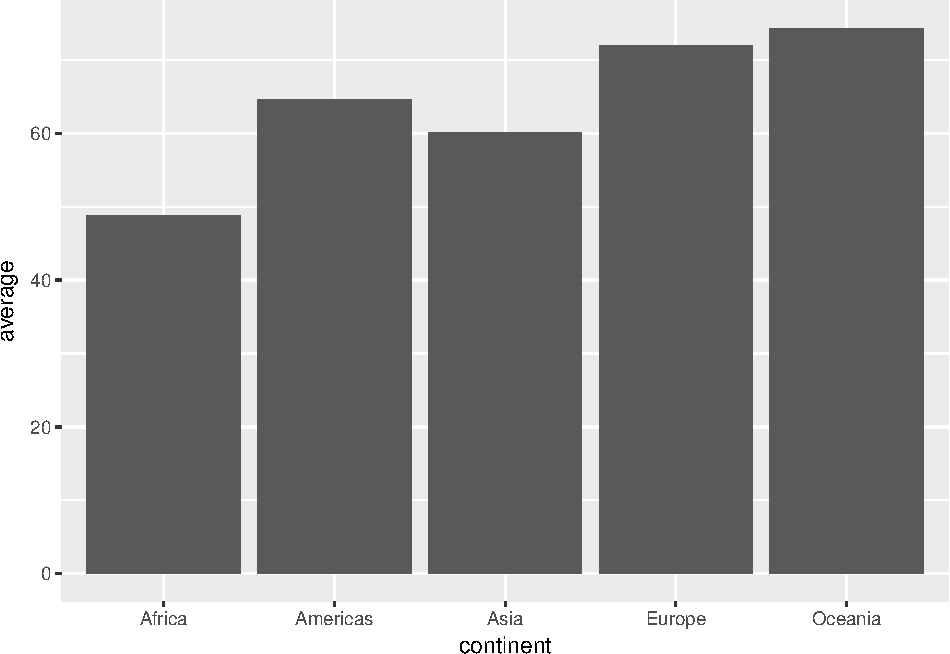
\includegraphics{Intro_data_wrangling_files/figure-latex/summ_cont-1.pdf}

\begin{Shaded}
\begin{Highlighting}[]
\NormalTok{(summ_year_life_exp <-}\StringTok{ }\NormalTok{data_gapminder }\OperatorTok
\StringTok{  }\NormalTok{dplyr}\OperatorTok{::}\KeywordTok{group_by}\NormalTok{(year) }\OperatorTok
\StringTok{  }\NormalTok{dplyr}\OperatorTok{::}\KeywordTok{summarise}\NormalTok{(}\DataTypeTok{average =} \KeywordTok{mean}\NormalTok{(lifeExp),}
                   \DataTypeTok{med =} \KeywordTok{median}\NormalTok{(lifeExp),}
                   \DataTypeTok{std =} \KeywordTok{sd}\NormalTok{(lifeExp),}
                   \DataTypeTok{variance =} \KeywordTok{var}\NormalTok{(lifeExp),}
                   \DataTypeTok{iqr =} \KeywordTok{IQR}\NormalTok{(lifeExp)}
\NormalTok{                   )}
\NormalTok{ )}
\end{Highlighting}
\end{Shaded}

\begin{verbatim}
## # A tibble: 12 x 6
##     year average   med   std variance   iqr
##    <int>   <dbl> <dbl> <dbl>    <dbl> <dbl>
##  1  1952    49.1  45.1  12.2     149.  20.7
##  2  1957    51.5  48.4  12.2     150.  21.8
##  3  1962    53.6  50.9  12.1     146.  21.8
##  4  1967    55.7  53.8  11.7     137.  21.4
##  5  1972    57.6  56.5  11.4     130.  20.7
##  6  1977    59.6  59.7  11.2     126.  19.9
##  7  1982    61.5  62.4  10.8     116.  18.0
##  8  1987    63.2  65.8  10.6     111.  16.9
##  9  1992    64.2  67.7  11.2     126.  16.5
## 10  1997    65.0  69.4  11.6     134.  18.5
## 11  2002    65.7  70.8  12.3     151.  19.9
## 12  2007    67.0  71.9  12.1     146.  19.3
\end{verbatim}

\begin{Shaded}
\begin{Highlighting}[]
\KeywordTok{ggplot}\NormalTok{(}\DataTypeTok{data =}\NormalTok{ summ_year_life_exp, }
       \KeywordTok{aes}\NormalTok{(}\DataTypeTok{x =}\NormalTok{ year, }\DataTypeTok{y =}\NormalTok{ average)) }\OperatorTok{+}\StringTok{ }
\StringTok{  }\KeywordTok{geom_point}\NormalTok{()}
\end{Highlighting}
\end{Shaded}

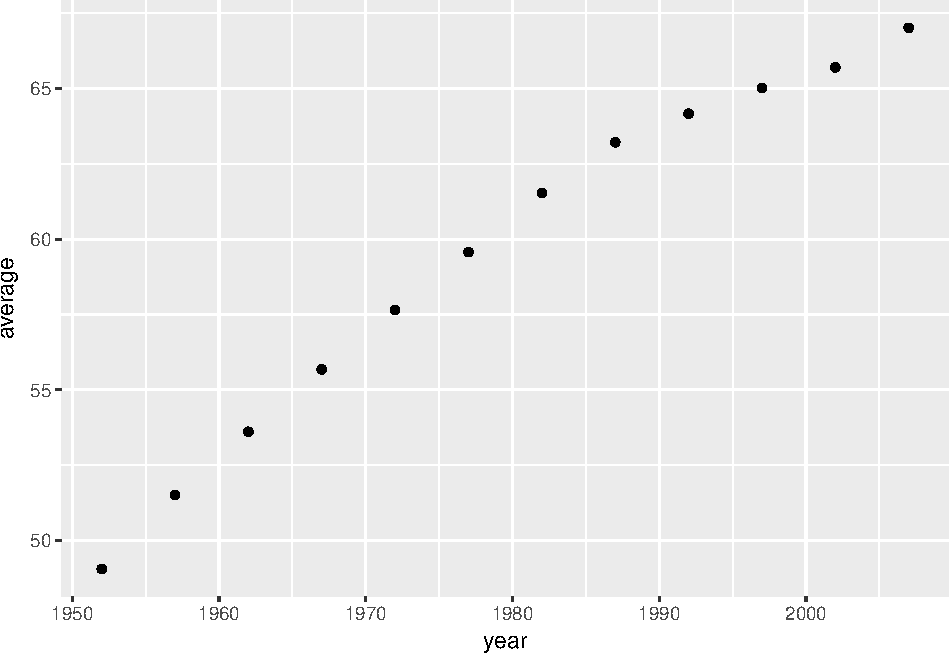
\includegraphics{Intro_data_wrangling_files/figure-latex/summ_cont-2.pdf}

One can also perform grouped mutates and grouped filters.


\end{document}
